\documentclass{standalone}
\usepackage{tikz}
\usetikzlibrary{patterns, positioning}


\begin{document}
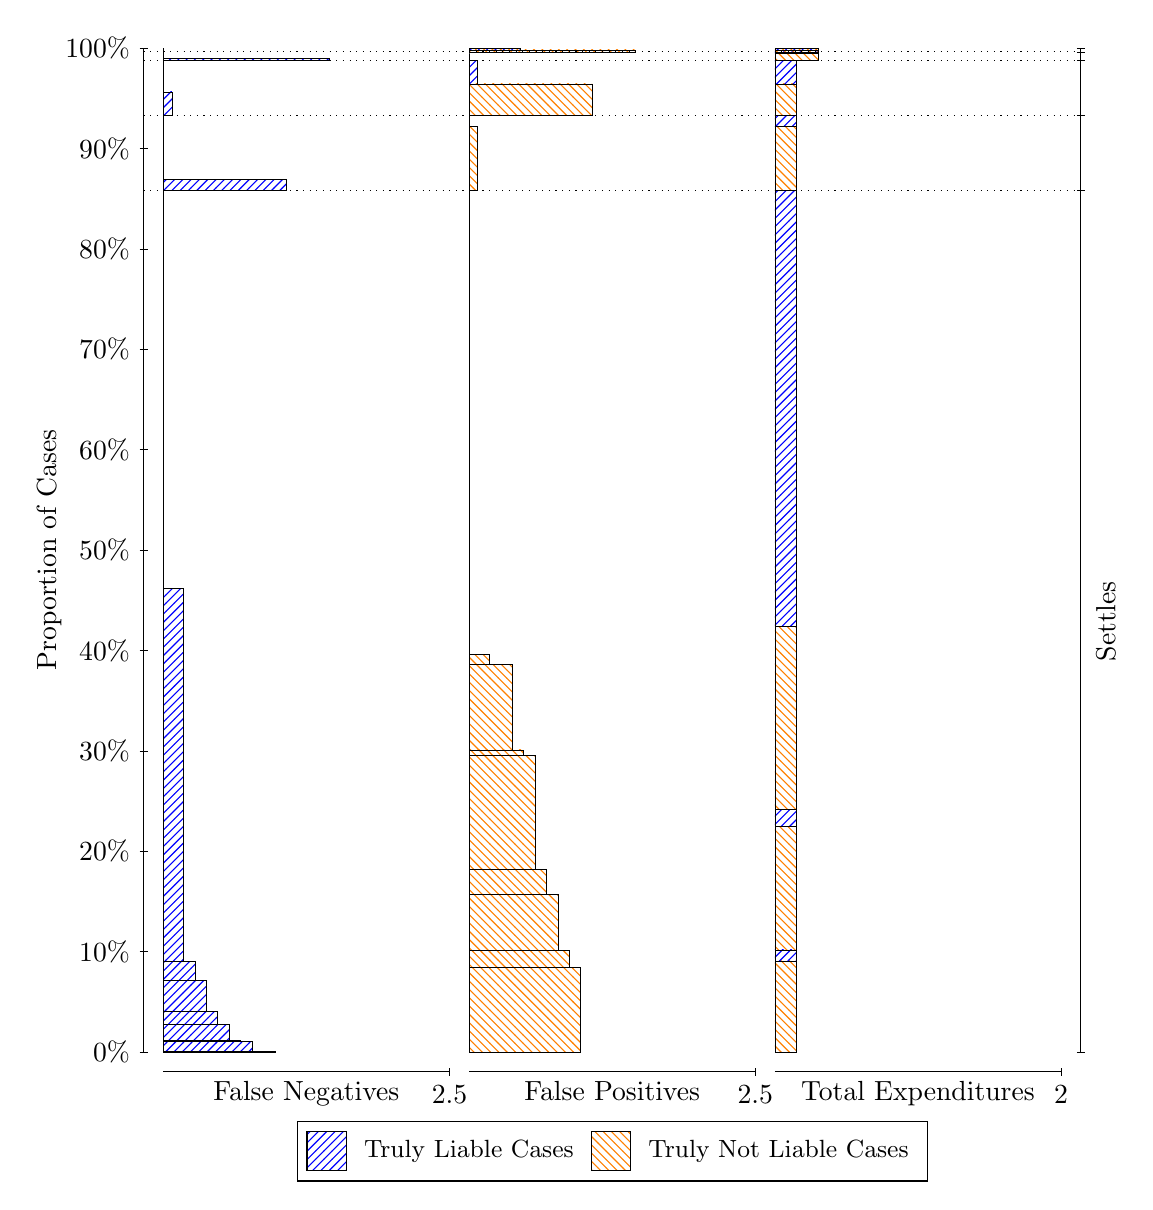
\begin{tikzpicture}
\draw[black, very thin] (1.5,1.75) -- (1.5,14.5);
\node[rotate=90, text=black, anchor=center] at (0.3, 8.125) {Proportion of Cases};
\draw[black, very thin] (1.45,1.75) -- (1.55,1.75);
\node[text=black, anchor=east] at (1.45, 1.75) {0\%};
\draw[black, very thin] (1.45,3.025) -- (1.55,3.025);
\node[text=black, anchor=east] at (1.45, 3.025) {10\%};
\draw[black, very thin] (1.45,4.3) -- (1.55,4.3);
\node[text=black, anchor=east] at (1.45, 4.3) {20\%};
\draw[black, very thin] (1.45,5.575) -- (1.55,5.575);
\node[text=black, anchor=east] at (1.45, 5.575) {30\%};
\draw[black, very thin] (1.45,6.85) -- (1.55,6.85);
\node[text=black, anchor=east] at (1.45, 6.85) {40\%};
\draw[black, very thin] (1.45,8.125) -- (1.55,8.125);
\node[text=black, anchor=east] at (1.45, 8.125) {50\%};
\draw[black, very thin] (1.45,9.4) -- (1.55,9.4);
\node[text=black, anchor=east] at (1.45, 9.4) {60\%};
\draw[black, very thin] (1.45,10.675) -- (1.55,10.675);
\node[text=black, anchor=east] at (1.45, 10.675) {70\%};
\draw[black, very thin] (1.45,11.95) -- (1.55,11.95);
\node[text=black, anchor=east] at (1.45, 11.95) {80\%};
\draw[black, very thin] (1.45,13.225) -- (1.55,13.225);
\node[text=black, anchor=east] at (1.45, 13.225) {90\%};
\draw[black, very thin] (1.45,14.5) -- (1.55,14.5);
\node[text=black, anchor=east] at (1.45, 14.5) {100\%};

\draw[black, very thin] (13.4,1.75) -- (13.4,14.5);
\draw[black, very thin] (13.35,1.75) -- (13.45,1.75);
\node[anchor=west] at (13.35, 1.75) {};
\draw[black, very thin] (13.35,12.691) -- (13.45,12.691);
\node[anchor=west] at (13.35, 12.691) {};
\draw[black, very thin] (13.35,13.647) -- (13.45,13.647);
\node[anchor=west] at (13.35, 13.647) {};
\draw[black, very thin] (13.35,14.341) -- (13.45,14.341);
\node[anchor=west] at (13.35, 14.341) {};
\draw[black, very thin] (13.35,14.452) -- (13.45,14.452);
\node[anchor=west] at (13.35, 14.452) {};
\draw[black, very thin] (13.35,14.5) -- (13.45,14.5);
\node[anchor=west] at (13.35, 14.5) {};

\draw[black, very thin, pattern color=blue, pattern=north east lines] (1.75,1.75) rectangle (3.167,1.7592);
\draw[black, very thin, pattern color=blue, pattern=north east lines] (1.75,1.7592) rectangle (2.8763,1.8887);
\draw[black, very thin, pattern color=blue, pattern=north east lines] (1.75,1.8887) rectangle (2.731,1.8963);
\draw[black, very thin, pattern color=blue, pattern=north east lines] (1.75,1.8963) rectangle (2.5857,2.1002);
\draw[black, very thin, pattern color=blue, pattern=north east lines] (1.75,2.1002) rectangle (2.4403,2.2621);
\draw[black, very thin, pattern color=blue, pattern=north east lines] (1.75,2.2621) rectangle (2.295,2.6546);
\draw[black, very thin, pattern color=blue, pattern=north east lines] (1.75,2.6546) rectangle (2.1497,2.8991);
\draw[black, very thin, pattern color=blue, pattern=north east lines] (1.75,2.8991) rectangle (2.0043,7.6398);
\draw[black, very thin, pattern color=orange, pattern=north west lines] (1.75,7.6398) rectangle (1.75,12.691);
\draw[black, very thin, pattern color=blue, pattern=north east lines] (1.75,12.691) rectangle (3.3123,12.832);
\draw[black, very thin, pattern color=orange, pattern=north west lines] (1.75,12.832) rectangle (1.75,13.647);
\draw[black, very thin, pattern color=blue, pattern=north east lines] (1.75,13.647) rectangle (1.859,13.944);
\draw[black, very thin, pattern color=orange, pattern=north west lines] (1.75,13.944) rectangle (1.75,14.341);
\draw[black, very thin, pattern color=blue, pattern=north east lines] (1.75,14.341) rectangle (3.8573,14.365);
\draw[black, very thin, pattern color=orange, pattern=north west lines] (1.75,14.365) rectangle (1.75,14.452);
\draw[black, very thin, pattern color=orange, pattern=north west lines] (1.75,14.452) rectangle (1.75,14.476);
\draw[black, very thin, pattern color=blue, pattern=north east lines] (1.75,14.476) rectangle (1.75,14.5);
\draw[black, very thin, pattern color=orange, pattern=north west lines] (5.6333,1.75) rectangle (7.0503,2.8223);
\draw[black, very thin, pattern color=orange, pattern=north west lines] (5.6333,2.8223) rectangle (6.905,3.0368);
\draw[black, very thin, pattern color=orange, pattern=north west lines] (5.6333,3.0368) rectangle (6.7597,3.7557);
\draw[black, very thin, pattern color=orange, pattern=north west lines] (5.6333,3.7557) rectangle (6.6143,4.0698);
\draw[black, very thin, pattern color=orange, pattern=north west lines] (5.6333,4.0698) rectangle (6.469,5.5171);
\draw[black, very thin, pattern color=orange, pattern=north west lines] (5.6333,5.5171) rectangle (6.3237,5.5873);
\draw[black, very thin, pattern color=orange, pattern=north west lines] (5.6333,5.5873) rectangle (6.1783,6.6753);
\draw[black, very thin, pattern color=orange, pattern=north west lines] (5.6333,6.6753) rectangle (5.8877,6.8011);
\draw[black, very thin, pattern color=blue, pattern=north east lines] (5.6333,6.8011) rectangle (5.6333,12.691);
\draw[black, very thin, pattern color=orange, pattern=north west lines] (5.6333,12.691) rectangle (5.7423,13.506);
\draw[black, very thin, pattern color=blue, pattern=north east lines] (5.6333,13.506) rectangle (5.6333,13.647);
\draw[black, very thin, pattern color=orange, pattern=north west lines] (5.6333,13.647) rectangle (7.1957,14.045);
\draw[black, very thin, pattern color=blue, pattern=north east lines] (5.6333,14.045) rectangle (5.7423,14.341);
\draw[black, very thin, pattern color=orange, pattern=north west lines] (5.6333,14.341) rectangle (5.6333,14.429);
\draw[black, very thin, pattern color=blue, pattern=north east lines] (5.6333,14.429) rectangle (5.6333,14.452);
\draw[black, very thin, pattern color=orange, pattern=north west lines] (5.6333,14.452) rectangle (7.7407,14.476);
\draw[black, very thin, pattern color=blue, pattern=north east lines] (5.6333,14.476) rectangle (6.2873,14.5);
\draw[black, very thin, pattern color=orange, pattern=north west lines] (9.5167,1.75) rectangle (9.7892,2.9082);
\draw[black, very thin, pattern color=blue, pattern=north east lines] (9.5167,2.9082) rectangle (9.7892,3.0454);
\draw[black, very thin, pattern color=orange, pattern=north west lines] (9.5167,3.0454) rectangle (9.7892,4.6185);
\draw[black, very thin, pattern color=blue, pattern=north east lines] (9.5167,4.6185) rectangle (9.7892,4.8316);
\draw[black, very thin, pattern color=orange, pattern=north west lines] (9.5167,4.8316) rectangle (9.7892,7.1513);
\draw[black, very thin, pattern color=blue, pattern=north east lines] (9.5167,7.1513) rectangle (9.7892,12.691);
\draw[black, very thin, pattern color=orange, pattern=north west lines] (9.5167,12.691) rectangle (9.7892,13.506);
\draw[black, very thin, pattern color=blue, pattern=north east lines] (9.5167,13.506) rectangle (9.7892,13.647);
\draw[black, very thin, pattern color=orange, pattern=north west lines] (9.5167,13.647) rectangle (9.7892,14.045);
\draw[black, very thin, pattern color=blue, pattern=north east lines] (9.5167,14.045) rectangle (9.7892,14.341);
\draw[black, very thin, pattern color=orange, pattern=north west lines] (9.5167,14.341) rectangle (10.062,14.429);
\draw[black, very thin, pattern color=blue, pattern=north east lines] (9.5167,14.429) rectangle (10.062,14.452);
\draw[black, very thin, pattern color=orange, pattern=north west lines] (9.5167,14.452) rectangle (10.062,14.476);
\draw[black, very thin, pattern color=blue, pattern=north east lines] (9.5167,14.476) rectangle (10.062,14.5);
\draw[black, dotted] (1.5,12.691) -- (13.4,12.691);
\draw[black, dotted] (1.5,13.647) -- (13.4,13.647);
\draw[black, dotted] (1.5,14.341) -- (13.4,14.341);
\draw[black, dotted] (1.5,14.452) -- (13.4,14.452);
\draw[black, very thin] (1.75,1.5) -- (5.3833,1.5);
\node[text=black, anchor=north] at (3.5667, 1.5) {False Negatives};
\draw[black, very thin] (5.3833,1.45) -- (5.3833,1.55);
\node[text=black, anchor=north] at (5.3833, 1.45) {2.5};

\draw[black, very thin] (5.6333,1.5) -- (9.2667,1.5);
\node[text=black, anchor=north] at (7.45, 1.5) {False Positives};
\draw[black, very thin] (9.2667,1.45) -- (9.2667,1.55);
\node[text=black, anchor=north] at (9.2667, 1.45) {2.5};

\draw[black, very thin] (9.5167,1.5) -- (13.15,1.5);
\node[text=black, anchor=north] at (11.333, 1.5) {Total Expenditures};
\draw[black, very thin] (13.15,1.45) -- (13.15,1.55);
\node[text=black, anchor=north] at (13.15, 1.45) {2};

\node[text=black, centered, rotate=90] at (13.72, 7.2205) {Settles};





\draw (7.449999999999999,1.5) node[draw=none] (baseCoordinate) {};
\begin{scope}[align=center]
        \matrix[scale=0.5, draw=black, below=0.5cm of baseCoordinate, nodes={draw}, column sep=0.1cm]{
            \node[rectangle, draw, minimum width=0.5cm, minimum height=0.5cm, pattern color=blue, pattern=north east lines] {}; &
            \node[draw=none, font=\small, text=black] (B) {Truly Liable Cases}; &
            \node[rectangle, draw, minimum width=0.5cm, minimum height=0.5cm, pattern color=orange, pattern=north west lines] {}; &
            \node[draw=none, font=\small, text=black] (B) {Truly Not Liable Cases}; \\
            };
\end{scope}

\end{tikzpicture}
\end{document}